\chapter{Applicazioni per il MM}\label{capitolo4}
In questo capitolo vengono spiegati i requisiti dei moduli sviluppati durante lo stage e la loro implementazione.
In particolare verranno esposte le dipendenze per il modulo dei comandi vocali (sezione \ref{cap:sox}), le metodologie
per accedere ai sevizi di Google (sezione \ref{cap:google}), come avviene la comunicazione tra l'API e il programma (sezione \ref{cap:api})
e l'implementazione del modulo con Touch Board (sezione \ref{cap:touch}).

\section{Modulo per comandi vocali}\label{cap:voce}
La prima applicazione implementata, come \`e stato accennato nell'introduzione del capitolo \ref{capitolo4}, \`e
stata il controllo del MagicMirror tramite comandi vocali.
Nello specifico l'applicazione deve, tramite delle specifiche frasi,
gestire le altre applicazioni presenti nel MagicMirror, sfruttando funzioni offerte dallo stesso.\\
Nella figura \ref{fig:modulovocale} \`e rappresentata la struttura e il funzionamento del modulo.
Il microfono cattura l'audio, che viene elaborato, all'interno del NodeHelper, dal software Sound eXchange (\textit{SoX}), un software per l'elaborazione e la manipolazione
dell'audio. Successivamente, l'audio così elaborato, viene
passato all'API Speech To Text, la quale lo inoltra al Servizio Google Speech e si mette in attesa di una risposta.
Al ritorno di questa, viene passata al modulo che ha il compito di validare il comando e di inoltrarlo ai moduli, se
corretto.
Per poter utilizzare l'API \`e necessario installare il software SoX e fornire un'autenticazione per i servizi Google.

\begin{figure}[H]
    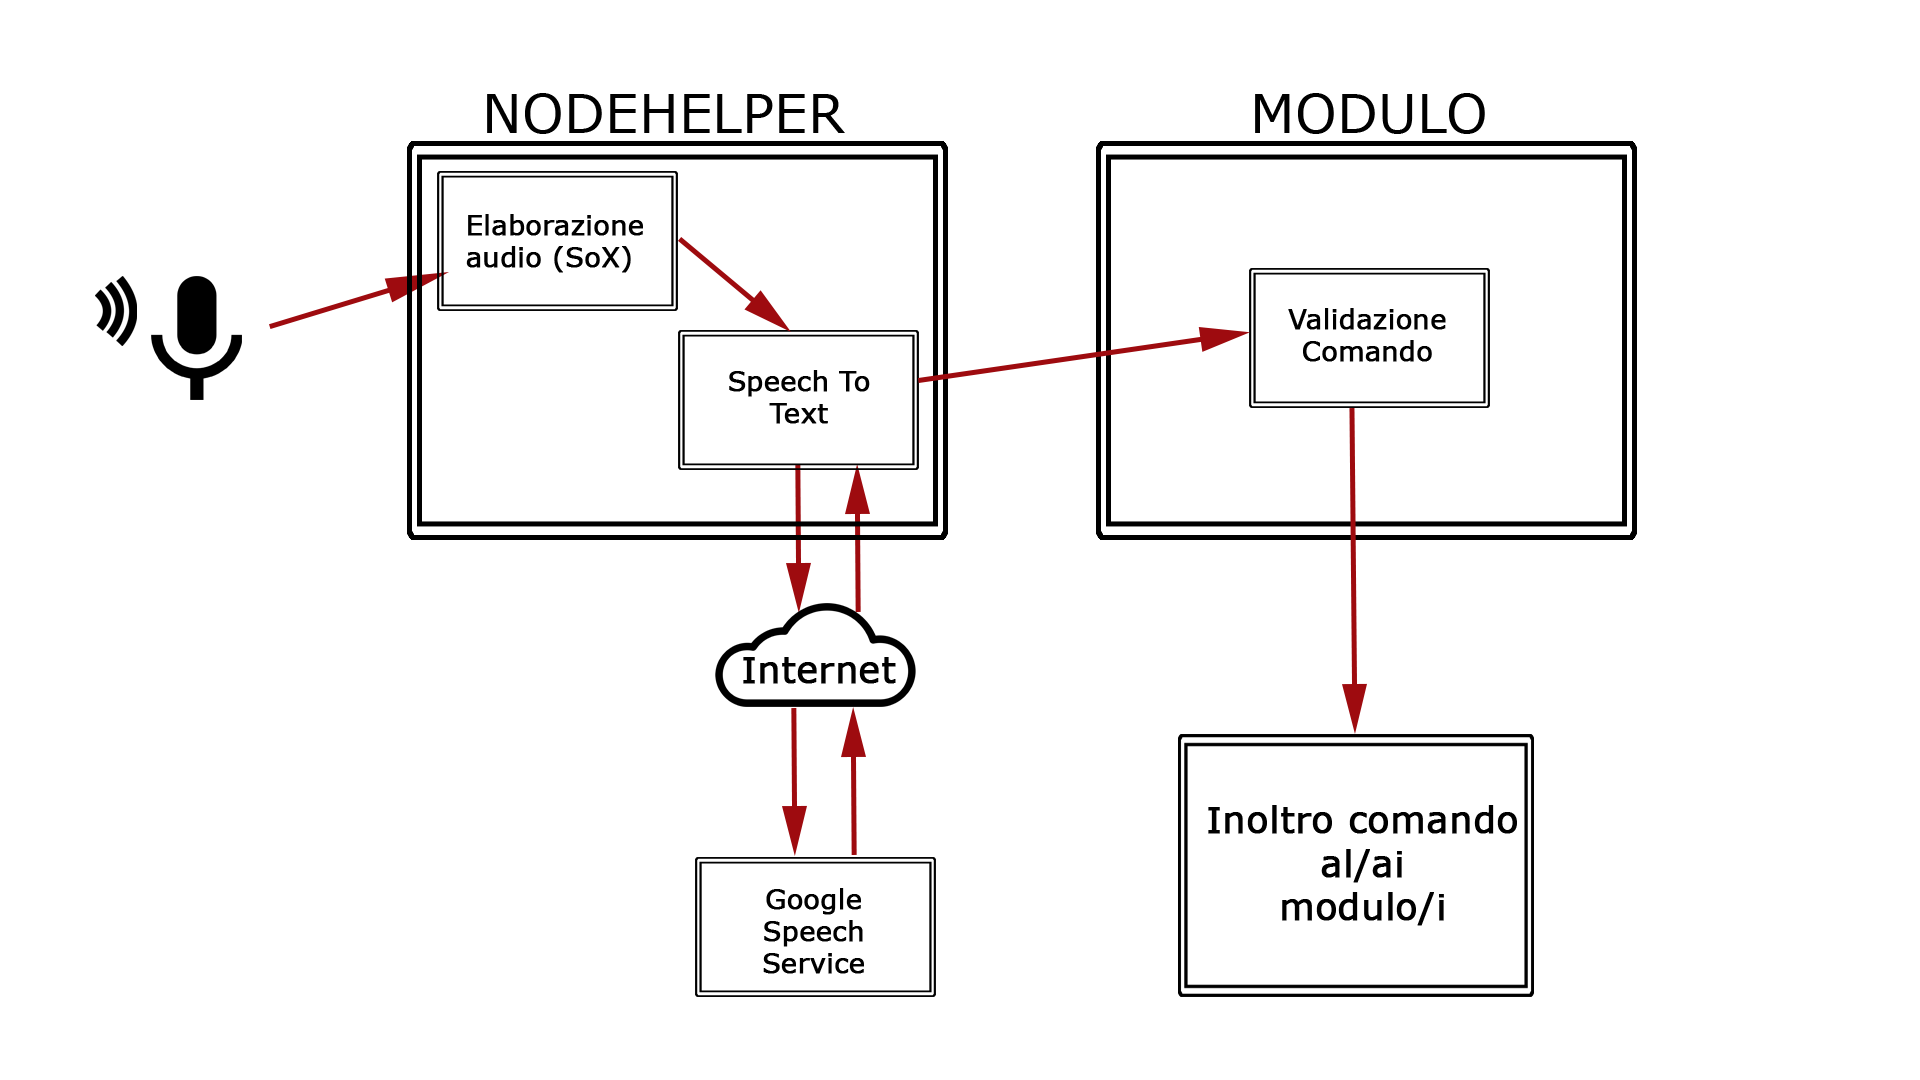
\includegraphics[width=1\textwidth, height=0.4\textheight]{modulovocale}
    \caption{Struttura del modulo per comandi vocali}
    \label{fig:modulovocale}
\end{figure}

\subsection{Comunicazione con l'API}\label{cap:api}
Il NodeHelper dell'applicazione si occupa di gestire lo streaming con l'API e
di mandare i risultati (o gli errori) all'applicazione tramite le funzioni messe
a disposizione dal MagicMirror, esposte nella sezione \ref{cap:MMmess}.
Il seguente codice viene usato per creare un canale streaming con l'API:
\begin{lstlisting}[language=Javascript, caption={Codice per l'inoltro dell'audio al Servizio Google}, captionpos=b]
      const recognizeStream = speech.streamingRecognize(request)
        .on('error', sendSocketNotification("error"))
        .on('data', (data) =>
          if(Transcription: ${data.results[0].alternatives[0].transcript})
            sendSocketNotification('limit_reached')
          else
            sendSocketNotification('response', data.results[0])
\end{lstlisting}
\emph{speech.streamingRecognize(request)}, richiama la funzione dell'API per aprire una connessione, dove \emph{request} \`e
il flusso audio.
La funzione si mette successivamente in attesa di una risposta dall'API la quale pu\`o essere di due tipi:
\begin{itemize}
\item errore, nel caso ci sia stato un errore di connessione. In questo caso viene mandato al modulo un messaggio di errore
\item dati di risposta, nel caso di risposta senza errori, ma che pu\`o essere divisa uteriormente in altre due risposte. La prima sia ha nel caso in cui
viene raggiunto il limite di parole tradotte (Google mette a disposizione un limite giornaliero per chi vuole usufruirne gratuitamente). In questo caso
il modulo lo notificherebbe a video con un messaggio di errore. La seconda risposta contiene una stringa con la frase tradotta,
che il modulo validerebbe come comando,
e, in caso di risposta positiva, la inoltrerebbe ai moduli.\\[1\baselineskip]
\end{itemize}
Per passare il flusso audio alla funzione appena descritta bisogna creare una \emph{pipe}, ovvero uno strumento
per permettere a due processi di comunicare.
Nel seguente codice:
\begin{lstlisting}[language=Javascript]
      // Start recording and send the microphone input to the Speech API
      record
        .start({
          sampleRateHertz: 1600,
          threshold: 0,
          verbose: false,
          recordProgram: 'sox',
          silence: '20.0'
        })
        .on('error', sendSocketNotification('error'))
        .pipe(recognizeStream);
\end{lstlisting}
\emph{record} \`e una funzione con ascolto di eventi che
imposta tramite il metodo \emph{.start} i settaggi dello streaming (per esempio la frequenza) e ne inizia la cattura.
L'evento \emph{.on('error')} serve per sollevare un'eccezione in caso di errore, che poi viene inoltrata al modulo.
L'evento \emph{.pipe(recognizeStream)} crea una pipe tra la funzione di registrazione e \emph{recognizeStream} descritta nel codice precedente,
passando il flusso audio direttamente alla funzione.

\subsection{Difficolt\`a incontrate}
\subsubsection{Sound eXchange (SoX)}\label{cap:sox}
Per permettere all'audio di venire correttamente elaborato
per lo streaming, \`e necessario utilizzare Sound eXchange (SoX), citato nella sezione \ref{cap:voce}.
Affinch\`e il microfono si colleghi correttamente al programma \`e necessario impostare correttamente
i valori delle varibili d'ambiente \textit{AUDIODEV} e \textit{AUDIODRIVER}.
La prima variabile corrisponde al dispositivo audio al quale il programma deve fare riferimento,
la seconda varibile al driver audio da utilizzare; di solito il predefinito \`e Advanced Linux Sound Architecture(ALSA).

\subsubsection{Autenticazione Google API}\label{cap:google}
Per poter usufruire delle API di Google \`e necessario fornire un'autenticazione a livello
di sistema.
Per poterlo fare bisogna ottenere delle credenziali di sicurezza per un account Google,
attivabili tramite Google Cloud Platform Console.
Le credenziali consistono in un username, l'email dell'account Google e una chiave di sicurezza unica,
 il tutto contenuto in un file JSON che pu\`o essere scaricato e salvato in locale.
Per poter permettere al sistema di utilizzare l'API occorre che il file JSON con le credenziali sia
raggiungibile all'interno del sistema e per rendere possibile ciò, bisogna creare una variabile d'ambiente con assegnato il percorso
dove si trova il file.

\section{Modulo con Touch Board}\label{cap:touch}
Nell'implementazione del modulo con la Touch Board \`e necessario aver installato nel sistema
il linguaggio di programmazione Python, descritto nella sezione \ref{cap:python}.\\
La Touch Board si presenta come una scheda con 40 porte I/O (le quali devono essere collegate alle
GPIO della scheda RaspberryPi) e con un sensore elettrico di prossimit\`a, come mostrato in figura \ref{fig:TouchBoard}, che permette di catturare i movimenti fino a
5 cm di distanza.
Le librerie Python, in dotazione con la scheda, offrono funzioni per catturare i diversi input trasmessi, come ad esempio
la direzione di spostamento del dito, oppure la cattura di un tocco sulla scheda.\\
La struttura del modulo, mostrata in figura \ref{fig:structtouch}, \`e composta da un'entit\`a che, al ricevimento di un input
sulla Touch Board, elabora e riconosce l'input ricevuto e lo inoltra al modulo.
Il comando viene validato e, in caso di risposta positiva, viene inoltrato agli altri moduli.
Per poter eseguire un programma Python sul MM \`e necessario usare la libreria Javascript \emph{Python-Shell}, la quale
permette di avviare una shell di Python in background e avviare, di conseguenza, i programmi.
La comunicazione tra programma Python e il NodeHelper avviene tramite messaggi in JSON. Quando la scheda riceve un input,
il programma Python comunica il risultato al NodeHelper che lo inoltra al modulo.

\begin{figure}[H]
    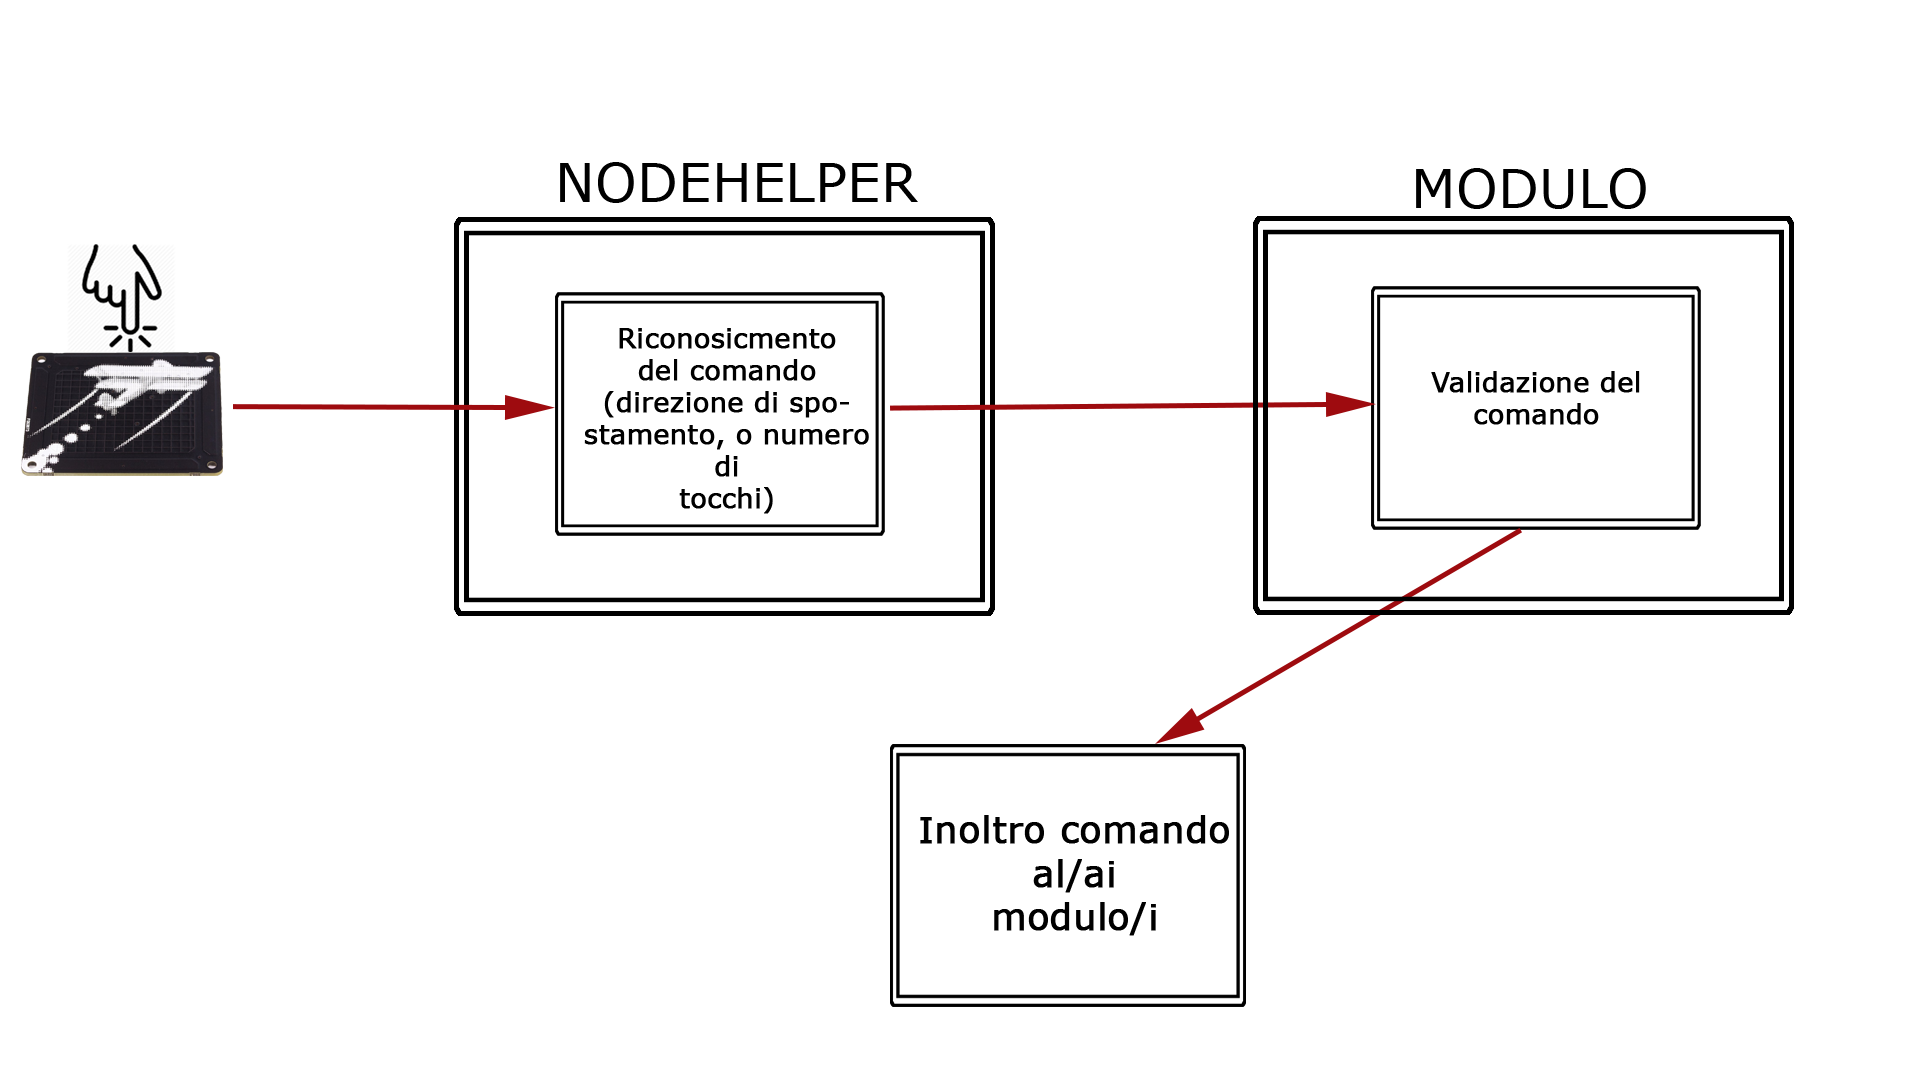
\includegraphics[width=1\textwidth, height=0.4\textheight]{touchstruct}
    \caption{Struttura del modulo con la Touch Board}
    \label{fig:structtouch}
\end{figure}

\begin{figure}[H]
    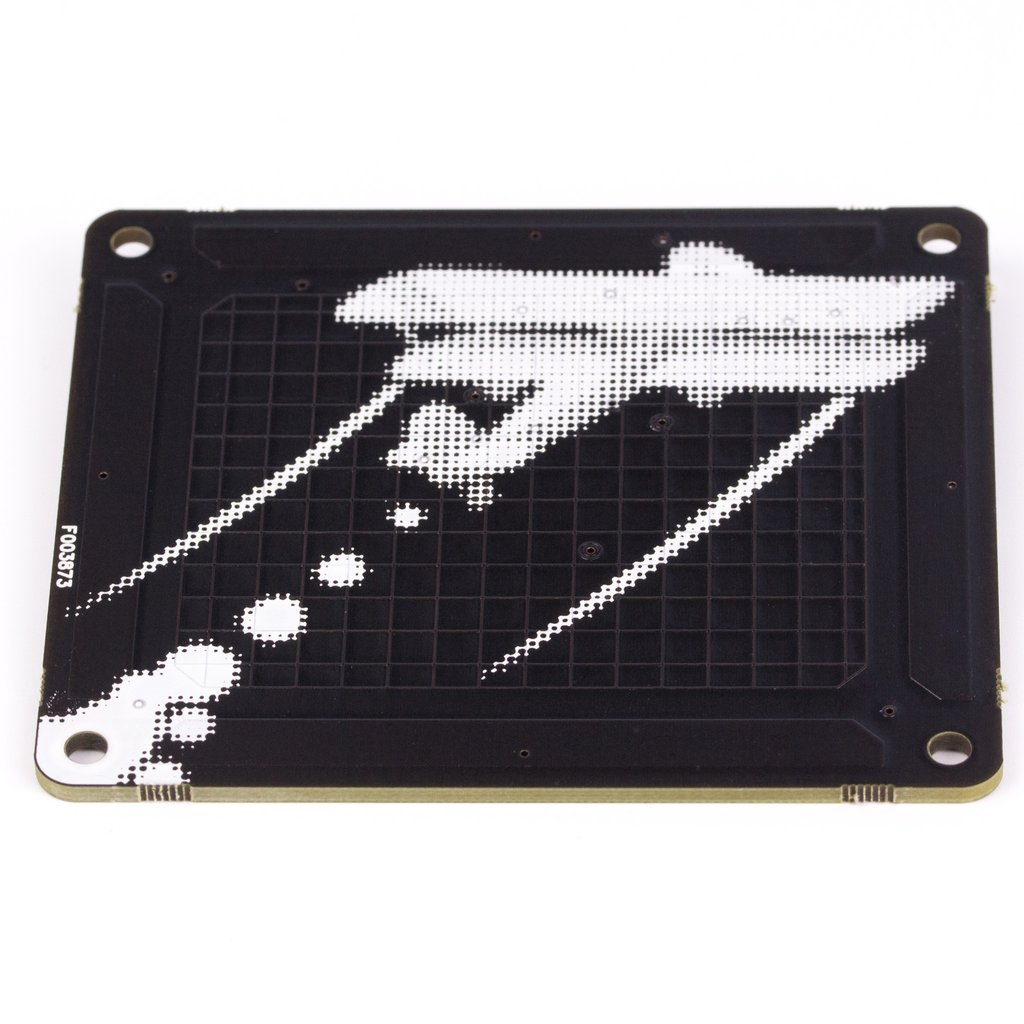
\includegraphics[width=1\textwidth, height=0.6\textheight]{skywriter}
    \caption{Touch Board Skydriver by Piromoni}
    \label{fig:TouchBoard}
\end{figure}
